\documentclass[a4paper]{article}

\input{style/ch_xelatex.tex}
\input{style/scala.tex}

\graphicspath{ {images/} }
\usepackage{ctex}
\usepackage{graphicx}
\usepackage{color,framed}%文本框
\usepackage{listings}
\usepackage{caption}

\usepackage{hyperref}
\hypersetup{hidelinks,
	colorlinks=true,
	allcolors=black,
	pdfstartview=Fit,
	breaklinks=true}


\usepackage{amssymb}
\usepackage{enumerate}
\usepackage{xcolor}
\usepackage{bm} 
\usepackage{lastpage}%获得总页数
\usepackage{fancyhdr}
\usepackage{tabularx}  
\usepackage{geometry}
\usepackage{minted}
\usepackage{graphics}
\usepackage{subfigure}
\usepackage{float}
\usepackage{pdfpages}
\usepackage{pgfplots}
\pgfplotsset{width=10cm,compat=1.9}
\usepackage{multirow}
\usepackage{footnote}
\usepackage{booktabs}
\usepackage{listings}
\usepackage{seqsplit}
\usepackage[table]{xcolor}
\usepackage{array}
%-----------------------伪代码------------------
\usepackage{algorithm}  
\usepackage{algorithmicx}  
\usepackage{algpseudocode}  
\floatname{algorithm}{Algorithm}  
\renewcommand{\algorithmicrequire}{\textbf{Input:}}  
\renewcommand{\algorithmicensure}{\textbf{Output:}} 
\usepackage{lipsum}  
\makeatletter
\newenvironment{breakablealgorithm}
  {% \begin{breakablealgorithm}
  \begin{center}
     \refstepcounter{algorithm}% New algorithm
     \hrule height.8pt depth0pt \kern2pt% \@fs@pre for \@fs@ruled
     \renewcommand{\caption}[2][\relax]{% Make a new \caption
      {\raggedright\textbf{\ALG@name~\thealgorithm} ##2\par}%
      \ifx\relax##1\relax % #1 is \relax
         \addcontentsline{loa}{algorithm}{\protect\numberline{\thealgorithm}##2}%
      \else % #1 is not \relax
         \addcontentsline{loa}{algorithm}{\protect\numberline{\thealgorithm}##1}%
      \fi
      \kern2pt\hrule\kern2pt
     }
  }{% \end{breakablealgorithm}
     \kern2pt\hrule\relax% \@fs@post for \@fs@ruled
  \end{center}
  }
\makeatother
%------------------------代码-------------------
\RequirePackage{listings}
\RequirePackage{xcolor}
\definecolor{dkgreen}{rgb}{0,0.6,0}
\definecolor{gray}{rgb}{0.5,0.5,0.5}
\definecolor{mauve}{rgb}{0.58,0,0.82}
\lstset{
	numbers=left,  
	frame=tb,
	aboveskip=3mm,
	belowskip=3mm,
	showstringspaces=false,
	columns=flexible,
	framerule=1pt,
	rulecolor=\color{gray!35},
	backgroundcolor=\color{gray!5},
	basicstyle={\ttfamily},
	numberstyle=\tiny\color{gray},
	keywordstyle=\color{blue},
	commentstyle=\color{dkgreen},
	stringstyle=\color{mauve},
	breaklines=true,
	breakatwhitespace=true,
	tabsize=3,
}

%-------------------------页面边距--------------
\geometry{a4paper,left=2.3cm,right=2.3cm,top=2.7cm,bottom=2.7cm}
%-------------------------页眉页脚--------------
\usepackage{fancyhdr}
\pagestyle{fancy}
\lhead{\kaishu 数据安全}
\chead{秘密共享与隐私计算实践} 
\rhead{2312966 林晖鹏}
\lfoot{}
\cfoot{\thepage}
\rfoot{}
\renewcommand{\headrulewidth}{0.1pt}  
\renewcommand{\footrulewidth}{0pt}
\newcommand{\HRule}{\rule{\linewidth}{0.5mm}}
\newcommand{\HRulegrossa}{\rule{\linewidth}{1.2mm}}
\setlength{\textfloatsep}{10mm}
\newcolumntype{Y}{>{\centering\arraybackslash\ttfamily}X}
\newcommand{\codewrap}[1]{\texttt{\seqsplit{#1}}}

\usepackage{indentfirst}  
\setlength{\parindent}{2em}  
\linespread{1.5}  

%--------------------文档内容--------------------

\begin{document}
\renewcommand{\contentsname}{目\ 录}
\renewcommand{\appendixname}{附录}
\renewcommand{\appendixpagename}{附录}
\renewcommand{\refname}{参考文献} 
\renewcommand{\figurename}{图}
\renewcommand{\tablename}{表}
\renewcommand{\today}{\number\year 年 \number\month 月 \number\day 日}

%-------------------------封面----------------

\renewcommand {\thefigure}{\thesection{}.\arabic{figure}}
\cfoot{\thepage\ of \pageref{LastPage}}

\newpage
\begin{center}
    \huge{\textbf{《数据安全》实验报告}}\\
    \vspace {0.5em}
    \Large {\textbf {秘密共享与隐私计算实践}}
\end{center}

\begin{center}
    \textbf{姓名}：\underline{林晖鹏} \quad
    \textbf{学号}：\underline{2312966} \quad
    \textbf{专业}：\underline{计算机科学与技术}
\end{center}

\vspace{1em} 

\tableofcontents

\newpage

%--------------------------Section 1--------------------------------
\section{实验要求}
本次实验旨在掌握 Shamir 秘密共享算法在隐私计算中的应用。本报告具体实现的内容包括：
\begin{enumerate}
    \item \textbf{实验 3.2 复现}：实现基于 $(2,3)$ 门限 Shamir 秘密共享的隐私投票系统，统计三个学生对四个候选人的投票结果，且不泄露个体投票信息。
    \item \textbf{扩展实验}：借鉴实验 3.2 的流程，实现三个参与方对其拥有的私有数据进行平均值计算的隐私协议，确保除最终平均值外，各方的私有数据不被泄露。
\end{enumerate}

%--------------------------Section 2--------------------------------
\section{实验原理}
\subsection{Shamir 秘密共享算法}
Shamir 秘密共享方案基于“两点确定一条直线，三点确定一条抛物线”的数学原理。对于 $(t, n)$ 门限方案：
\paragraph{分割阶段:}秘密 $S$ 被隐藏在一个 $t-1$ 次随机多项式的常数项中：
    \[ f(x) = S + a_1x + a_2x^2 + \dots + a_{t-1}x^{t-1} \pmod p \]
    生成 $n$ 个份额 $(i, f(i))$ 分发给各参与方。
\paragraph{重构阶段:} 任意 $t$ 个份额即可通过 \textbf{拉格朗日插值公式} 恢复秘密 $S$：
    \[ S = f(0) = \sum_{i=1}^{t} y_i \prod_{j=1, j \neq i}^{t} \frac{-x_j}{x_i - x_j} \pmod p \]

\subsection{秘密共享的加法同态性}
秘密共享方案具有线性性质，即“份额之和等于和的份额”。设参与方 $P_k$ 持有数据 $x_k$，其对应的份额为 $f_k(i)$。若各参与方在相同位置 $i$ 对份额进行累加：
\[ F(i) = \sum_{k=1}^m f_k(i) \]
则 $F(i)$ 构成了总和 $X = \sum x_k$ 的一个有效份额。通过重构 $F(0)$，可以在不泄露单个 $x_k$ 的前提下获得总和 $X$。

\subsection{隐私均值计算协议}

\begin{figure}[htbp]
    \centering
    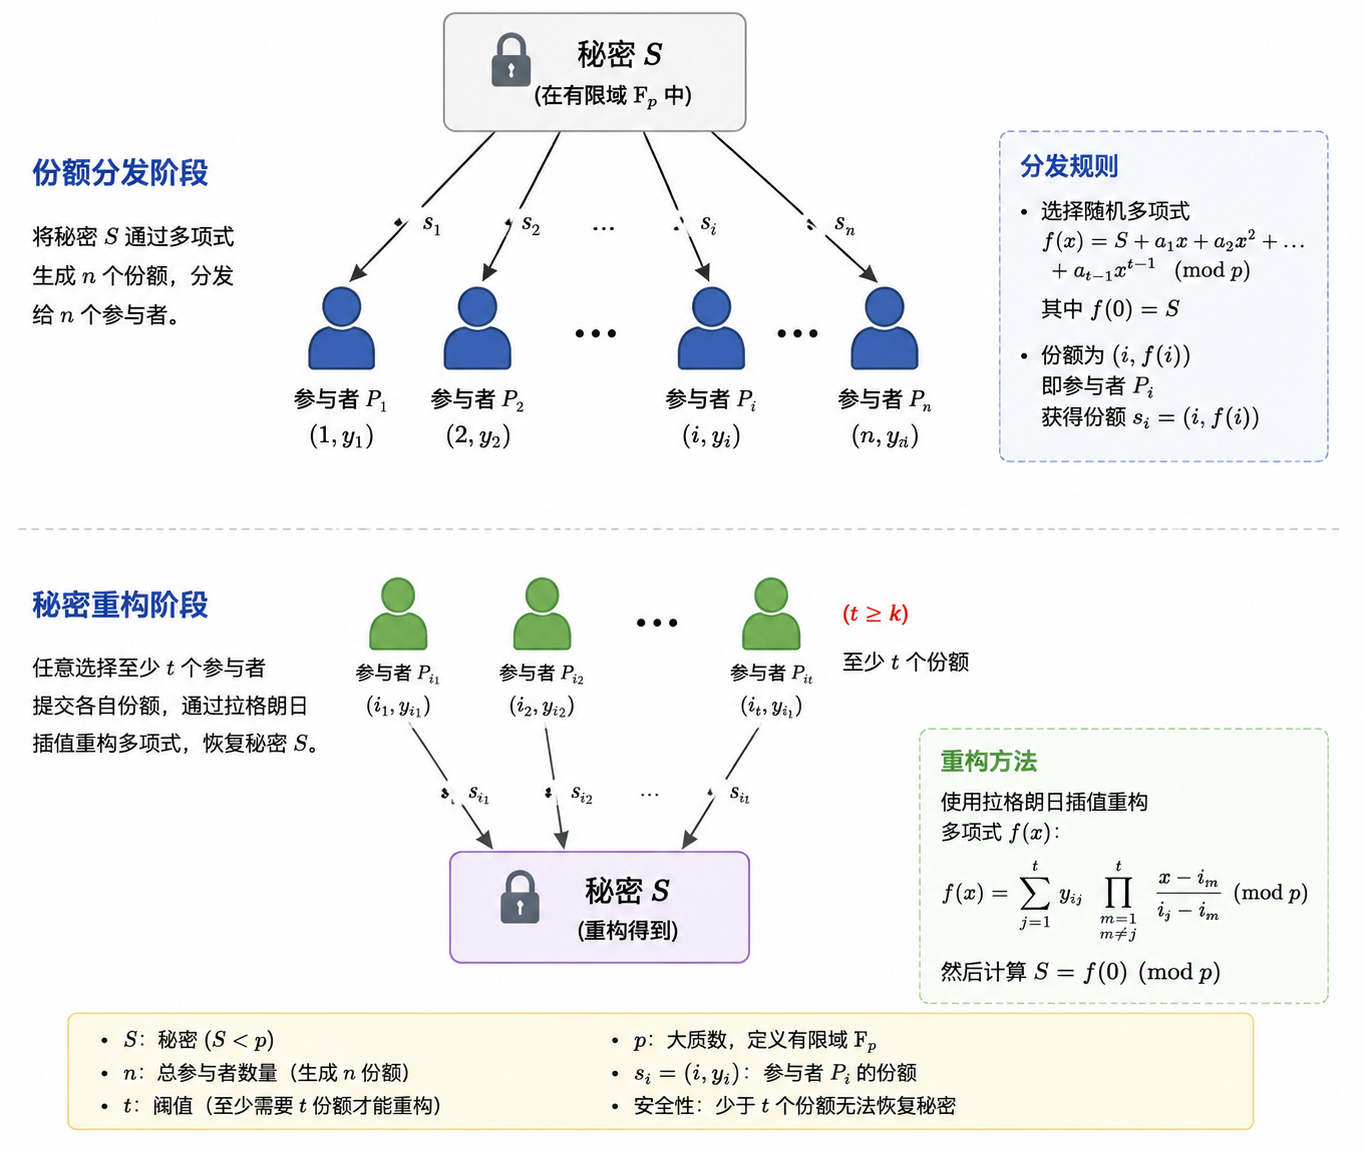
\includegraphics[width=0.8\textwidth]{image.png}
    \caption{协议示意图}
    \label{fig:privacy_mean}
\end{figure}


基于加法同态性，隐私均值计算流程如下：
\begin{enumerate}
    \item \textbf{秘密分割}：每个参与方将自己的私有数据 $x_k$ 生成 3 个份额。
    \item \textbf{份额交换}：参与方交换份额，使得每人持有所有数据在特定位置的份额。
    \item \textbf{本地累加}：每人计算手头份额之和 $d_i$。
    \item \textbf{重构与求均}：汇总 $d_i$ 并重构出总和 $X$，最后计算 $\bar{X} = X/m$。
\end{enumerate}

更具体、直白地说，比如设三位参与方分别持有私有数据 $x_1,x_2,x_3$。第 $k$ 位参与方会构造一个一次多项式
\[
f_k(x)=x_k+a_kx \pmod p,
\]
并在 $x=1,2,3$ 三个位置上分别计算函数值，从而得到三个点
\[
(1,f_k(1)),\quad (2,f_k(2)),\quad (3,f_k(3)).
\]
随后，参与方之间按照点的横坐标进行交换：第一位参与方最终收集到 $f_1(1),f_2(1),f_3(1)$，第二位参与方收集到 $f_1(2),f_2(2),f_3(2)$，第三位参与方收集到 $f_1(3),f_2(3),f_3(3)$。这样一来，每个人手里都只持有“综合函数”在某一个位置上的取值，而不是任何一方的原始数据。

接下来，各参与方分别在本地把自己收到的三个值相加，得到
\[
d_1=f_1(1)+f_2(1)+f_3(1),\quad
d_2=f_1(2)+f_2(2)+f_3(2),\quad
d_3=f_1(3)+f_2(3)+f_3(3).
\]
实际上，$d_1,d_2,d_3$ 正好对应于总和多项式
\[
F(x)=f_1(x)+f_2(x)+f_3(x)
\]
在 $x=1,2,3$ 处的三个函数值，而该多项式在 $x=0$ 处的值满足
\[
F(0)=x_1+x_2+x_3.
\]
因此，只需从 $d_1,d_2,d_3$ 中任选两个值进行拉格朗日插值，就可以恢复出三人数据的总和，最后再除以参与方人数 $3$，即可得到平均值。整个过程中被公开的始终只是份额和重构结果，单个参与方的私有输入不会直接暴露。

%--------------------------Section 3--------------------------------
\section{实验过程}

\subsection{核心算法实现}
实验采用了大质数 $p = 2^{31}-1$ 构建有限域，确保所有加法、乘法与插值运算都在模 $p$ 的意义下进行。这样做一方面可以避免普通整数计算中数值过大的问题，另一方面也符合秘密共享方案在有限域上的理论要求。

为了在程序中复现 Shamir 秘密共享协议，这里将整个逻辑抽象为“分发”与“重构”两个核心阶段。具体来说，\texttt{generate\_shares} 函数扮演了“分发者”的角色，它负责将每个人的私密原始数据打碎，转化为一系列看似随机的份额点；而 \texttt{reconstruct\_secret} 函数则扮演了“收割者”的角色，只要凑齐了足够门限数量的份额，它就能通过数学插值把藏在背后的秘密算出来。

\begin{lstlisting}[language=Python,caption={Shamir 秘密共享核心实现}]
def generate_shares(secret, n, t):
    # 把秘密藏在常数项，剩下的系数随便抓点随机数填充
    coefficients = [secret] + [random.randint(0, PRIME - 1) for _ in range(t - 1)]
    def f(x):
        result = 0
        # 按照多项式 f(x) = a0 + a1*x + a2*x^2 ... 的样子算一遍
        for i, coeff in enumerate(coefficients):
            result = (result + coeff * pow(x, i, PRIME)) % PRIME
        return result
    # 给 n 个人每人发一个坐标点 (x, f(x))
    return [(i, f(i)) for i in range(1, n + 1)]

def reconstruct_secret(shares):
    # 把大家手里拿到的 (x, y) 点集拆开
    x_values, y_values = zip(*shares)
    def lagrange(x):
        total = 0
        for i in range(len(x_values)):
            num, den = 1, 1
            for j in range(len(x_values)):
                if i == j: continue
                # 拉格朗日基函数的分子分母，这里纯纯是数学公式搬运
                num = (num * (x - x_values[j])) % PRIME
                den = (den * (x_values[i] - x_values[j])) % PRIME
            # 在有限域里，“除法”得通过逆元来实现，这就体现出质数 PRIME 的作用了
            term = (y_values[i] * num * pow(den, -1, PRIME)) % PRIME
            total = (total + term) % PRIME
        return total
    # 算 f(0) 其实就是在拿多项式的常数项
    return lagrange(0)
\end{lstlisting}

首先来看 \texttt{generate\_shares} 的实现。该函数的输入分别是秘密值 \texttt{secret}、份额总数 \texttt{n} 和门限值 \texttt{t}。在本实验中采用的是 $(2,3)$ 门限，因此 \texttt{t=2}、\texttt{n=3}，对应的多项式就是一次多项式。代码中的
\[
\texttt{coefficients = [secret] + [random.randint(0, PRIME - 1) for \_ in range(t - 1)]}
\]
表示将秘密值作为多项式的常数项，再随机生成其余系数。这样构造出的多项式既包含真实秘密，又由于随机系数的加入而具有隐藏性。

随后，函数内部定义了一个匿名的多项式求值过程 \texttt{f(x)}。它的作用是在给定横坐标 $x$ 的情况下，计算多项式在该点的函数值。代码中通过
\[
\sum_i a_i x^i \bmod p
\]
的形式逐项累加，从而得到 $f(1), f(2), \dots, f(n)$。对于本实验而言，也就是生成三个点 $(1,f(1))$、$(2,f(2))$ 和 $(3,f(3))$。这三个点就是要分发给不同参与方的秘密份额。

接下来我们继续分析 \texttt{reconstruct\_secret} 函数。它接收若干个份额点 \texttt{shares}，并尝试恢复多项式在 $x=0$ 处的函数值。由于秘密被定义为多项式的常数项，因此只要求出 $f(0)$，就等价于恢复原始秘密。

这里采用的方法是拉格朗日插值。代码先把份额拆分为横坐标序列 \texttt{x\_values} 和纵坐标序列 \texttt{y\_values}，然后在内部函数 \texttt{lagrange(x)} 中逐项构造插值基函数。对于每一个已知点 $(x_i, y_i)$，程序都会计算其对应的插值权重，并将所有项加总起来，最终得到目标点处的函数值。当调用 \texttt{lagrange(0)} 时，就意味着在求多项式的截距，也就是秘密本身。

这里需要特别说明的是，拉格朗日插值公式中存在除法，而在有限域中不能直接使用普通实数除法，因此代码中通过 \texttt{pow(den, -1, PRIME)} 计算分母在模 $p$ 下的逆元，再将除法转化为乘法完成运算。这也是有限域插值实现中的关键步骤。

从整体上看，这段核心代码完整对应了 Shamir 秘密共享方案的数学过程：先将秘密编码为随机多项式，再通过若干点分发份额；当收集到不少于门限数量的点后，再利用插值方法恢复出原始秘密。

\subsection{实验 3.2 复现：隐私投票模拟流程详解}
在上一小节熟悉了核心算法的基础上，本小节结合投票模拟的完整代码，逐一讲解如何利用秘密共享实现四人投票的隐私统计。整个流程大致可以分为四个阶段。

\textbf{第一步：初始化投票矩阵。} 程序在本地定义了一个 $3 \times 4$ 的投票矩阵 \texttt{actual\_votes}，每一行对应一位学生的投票意向，每一列对应一位候选人。投票值只有 0 和 1 两种，分别代表"反对"和"赞成"。与此同时，代码还准备了一个 \texttt{theoretical\_results} 列表，用直接相加的方式算出每位候选人的理论得票数，后面用来验证隐私计算的结果是否正确。

\textbf{第二步：对每一张选票做秘密分割。} 这里用一个三层嵌套的循环来完成。具体来说，外层循环遍历四个候选人，中层循环遍历三个学生，内层则调用 \texttt{generate\_shares}，把学生投出的那张选票（0 或 1）转换成三个份额点。拿 Student 1 给 Alice 投的 1 票来说，这张票会被编码为一个一次多项式 $f(x)=1+a_1x \pmod p$，然后计算出三个点 $(1,f(1))$、$(2,f(2))$、$(3,f(3))$。这三个点分别交给投票员手里的不同位置，供后续汇总使用。所有票的份额最终存入 \texttt{all\_shares} 三维列表中。

\begin{lstlisting}[language=Python,caption={秘密分割核心代码片段}]
# 为每个候选人的每一票生成 3 个份额
all_shares = [[[] for _ in range(3)] for _ in range(4)]

for c_idx in range(4):
    for s_idx in range(3):
        vote = actual_votes[s_idx][c_idx]
        shares = generate_shares(vote, 3, 2)  # (2,3) 门限
        all_shares[c_idx][s_idx] = shares
\end{lstlisting}

\textbf{第三步：模拟投票员汇总份额。} 投票员并不直接接触任何一张原始选票，他手里只有所有学生提交上来的份额。在这一步，程序模拟投票员对每个候选人分别做按位置累加。例如，对于 Alice 这位候选人，投票员把 Student 1、2、3 在 $x=1$ 处的份额相加，得到 $d_1$；在 $x=2$ 处的份额相加，得到 $d_2$；在 $x=3$ 处的份额相加，得到 $d_3$。这一步的数学意义在于：由于 Shamir 份额天然满足加法同态，$d_1,d_2,d_3$ 实际上就是"总和多项式" $F(x)=f_1(x)+f_2(x)+f_3(x)$ 在 $x=1,2,3$ 处的函数值，而 $F(0)$ 恰好等于 Alice 的总票数。

\begin{lstlisting}[language=Python,caption={份额汇总核心代码片段}]
final_candidate_shares = []
for c_idx in range(4):
    candidate_sum_shares = []
    for x_val in range(1, 4):
        total_y_at_x = sum(
            all_shares[c_idx][s_idx][x_val-1][1] for s_idx in range(3)
        ) % PRIME
        candidate_sum_shares.append((x_val, total_y_at_x))
    final_candidate_shares.append(candidate_sum_shares)
\end{lstlisting}

\textbf{第四步：重构票数。} 投票员从 $d_1,d_2,d_3$ 中随机抽取两个（比如 $d_1$ 和 $d_3$），调用 \texttt{reconstruct\_secret} 进行拉格朗日插值。由于插值公式可以唯一确定一条直线，而这条直线的截距正好是 $F(0)$，所以只要有两个点就能把票数还原出来。程序对四位候选人都执行同样的操作，最终得到所有人的得票结果。

\begin{lstlisting}[language=Python,caption={票数重构核心代码片段}]
reconstructed_results = []
for c_idx in range(4):
    subset_shares = random.sample(final_candidate_shares[c_idx], 2)
    total_votes = reconstruct_secret(subset_shares)
    reconstructed_results.append(total_votes)
    print(f"候选人 {candidates[c_idx]:7}: {total_votes} 票")
\end{lstlisting}

\subsection{隐私计算模拟逻辑详解}
在投票实验的基础上，本小节进一步将同样的思路迁移到连续值（成绩）的场景，讲解如何利用秘密共享计算三个学生私有数据的平均值。整体框架与投票实验几乎完全一致，只是在具体数据和最后一步的处理上有所不同。

\textbf{第一步：准备三个人的私有数据。} 与投票场景不同，这里每个人的数据不再是只能取 0 或 1 的离散值，而是一个任意的整数。程序定义了 \texttt{student\_data = [60, 80, 100]}，分别代表三位同学各自的数据（比如可以是成绩或其他敏感数值）。同时计算出理论总和与理论平均值，方便后面做验证。

\textbf{第二步：每个人都把自己的数据藏进一条直线里。} 这里没有像投票那样三层循环嵌套，而是直接对三个学生各自调用一次 \texttt{generate\_shares}。拿 Student 1 的数据 $60$ 来说，程序会随机生成一条过 $(0,60)$ 的一次直线 $f_1(x)=60+a_1x \pmod p$，然后算出三个点 $(1,f_1(1))$、$(2,f_1(2))$、$(3,f_1(3))$。这三个点虽然看起来毫无规律，但只要任意两个凑在一起，就能把 $60$ 还原出来。三个人的份额分别存入 \texttt{shares\_matrix}，打印出来可以看到每个学生的份额都不一样，这正是因为随机斜率导致的。

\begin{lstlisting}[language=Python,caption={份额生成代码片段}]
shares_matrix = []
for i, data in enumerate(student_data):
    shares = generate_shares(data, 3, 2)
    shares_matrix.append(shares)
    print(f"{names[i]} 生成的份额: {shares}")
\end{lstlisting}

\textbf{第三步：模拟投票员把所有份额按位置相加。} 程序用一个 \texttt{for j in range(3)} 循环，依次在 $x=1,2,3$ 三个位置把所有学生的份额纵向相加。例如在 $x=1$ 处，把 Student 1 的 $f_1(1)$、Student 2 的 $f_2(1)$、Student 3 的 $f_3(1)$ 加在一起得到 $d_1$；同理得到 $d_2$ 和 $d_3$。从数学上看，$d_1,d_2,d_3$ 就是综合多项式 $F(x)=f_1(x)+f_2(x)+f_3(x)$ 在 $x=1,2,3$ 处的函数值，而 $F(0)=60+80+100=240$，这恰好就是三个人的数据总和。

\begin{lstlisting}[language=Python,caption={份额按位置汇总代码片段}]
sum_shares = []
for j in range(3):
    local_sum = sum(
        shares_matrix[i][j][1] for i in range(3)
    ) % PRIME
    sum_shares.append((j + 1, local_sum))
print(f"投票员累加后的总份额 (d1, d2, d3): {sum_shares}")
\end{lstlisting}

\textbf{第四步：用两个点把总和还原出来，再除以人数得到平均值。} 程序直接取了前两个汇总份额作为重构的输入，送入 \texttt{reconstruct\_secret} 中做拉格朗日插值。由于这两个点可以唯一确定那条综合直线，所以直接能算出截距 $F(0)=240$。最后把 $240$ 除以 $3$，就得到了三位同学的平均成绩 $80.0$。与理论值对比验证无误，说明整个隐私计算流程是正确运行的。

\begin{lstlisting}[language=Python,caption={重构与求均值代码片段}]
reconstruction_shares = sum_shares[:2]
reconstructed_sum = reconstruct_secret(reconstruction_shares)
reconstructed_avg = reconstructed_sum / 3
print(f"重构出的总和: {reconstructed_sum}")
print(f"最终计算出的平均值: {reconstructed_avg:.2f}")
\end{lstlisting}

%--------------------------Section 4--------------------------------
\section{实验结果与分析}
\subsection{隐私均值计算结果}
运行程序，输出结果如下：
\begin{lstlisting}[caption={隐私均值计算实验输出}]
--- 三人数据平均值隐私计算模拟 ---
原始数据: {'Student 1': 60, 'Student 2': 80, 'Student 3': 100}
理论总和: 240, 理论平均值: 80.00
--------------------------------------------------
Student 1 生成的份额: [(1, 1883659394), (2, 1619835081), (3, 1356010768)]
...
投票员累加后的总份额 (d1, d2, d3): [(1, 1467640431), (2, 787796975), (3, 107953519)]
重构出的总和: 240
最终计算出的平均值: 80.00
验证成功：隐私计算结果与直接计算一致！
\end{lstlisting}

从输出可以看出，三个人的原始数据分别为 60、80 和 100，理论总和为 240，平均值为 80.00。在隐私计算阶段，每个人独立生成自己的多项式份额，打印出的三行份额分别对应三位学生的随机直线在 $x=1,2,3$ 处的取值，彼此之间毫无规律可循。投票员将所有人同一位置的份额相加后，得到 $d_1,d_2,d_3$ 三个聚合值。最后通过拉格朗日插值还原出总和 240，除以 3 得到平均值 80.00，与理论值完全一致。整个过程中，任何人都无法从中间结果反推出原始的个人数据。

\subsection{实验 3.2 隐私投票结果}
运行程序，输出结果如下：
\begin{lstlisting}[caption={投票系统实验输出}]
--- 实验 3.2：基于 Shamir (2,3) 门限的隐私投票系统 ---
原始投票情况：
          Alice  Bob  Charles  Douglas
Student 1:  1      0      1      1
Student 2:  0      1      1      0
Student 3:  1      1      0      1
------------------------------------------------------------
投票员汇总后的部分份额展示（仅展示 Alice 的前两个份额）：
Alice"'"s aggregated shares (subset): [(1, 1043356503), (2, 2086713004)]
------------------------------------------------------------
最终统计结果：
候选人 Alice  : 2 票
候选人 Bob    : 2 票
候选人 Charles: 2 票
候选人 Douglas: 2 票
------------------------------------------------------------
验证成功：隐私统计的总票数与直接相加结果完全一致！
\end{lstlisting}

从结果可以看出，三位同学对四位候选人的投票矩阵经过秘密分割与分布式汇总后，最终每位候选人的得票均被正确还原为 2 票。由于在份额汇总阶段采用的是 $(2,3)$ 门限，投票员实际上只掌握了 $d_1,d_2,d_3$ 三个聚合值，这些值本身并不包含任何单一学生的投票信息，从而实现了投票的隐私保护。

\subsection{安全性分析}
\begin{enumerate}
    \item \textbf{隐私保护}：实验中，原始数据仅作为多项式的常数项存在。在有限域 $GF(p)$ 下，由于随机系数的存在，单个份额对于攻击者而言是均匀分布的随机值，不包含任何关于秘密的信息。
    \item \textbf{容错性}：由于采用 $(2,3)$ 门限，即使其中一个参与方的份额丢失或网络故障，只要剩余两个参与方协作，仍能正确完成计算。
\end{enumerate}

%--------------------------Section 5--------------------------------
\section{总结与感想}
本次实验通过动手实践，深入理解了 Shamir 秘密共享这一经典隐私计算协议。实验中最深刻的体会是秘密共享方案的“线性”特征——这种特征使得我们能够在密文（份额）上直接进行算术运算，其结果在解密后依然保持逻辑一致性。

这种“运算而无感知”的特性是多方安全计算（MPC）的基石。在未来的数据安全应用中，这种技术可以广泛应用于敏感数据的联合统计、金融风控等领域，真正实现“数据可用不可见”。

\end{document}
